\title{The Battle of Surrey's Wards}
\author{Sepideh Nazemi}
\date{}
\documentclass[12pt]{article}
\usepackage{graphicx}
\usepackage{hyperref}
\usepackage{footnote}
\makesavenoteenv{tabular}
\begin{document}
\maketitle
\section{Introduction}
\subsection{Background}
Buying a house has always been a great adventure, especially when it is the first home. However, at the same time, it can be very challenging too. Finding a proper location to buy a house is not a straightforward task. Many factors need to be considered to analyse and compare different locations suitability. For example, closeness to the workplace, kids' schools or leisure centres, safety and accessibility to hospitals, public transport or motorways can be the critical factors. The list is not exhaustive. The problem gets more challenging than ever if you are new to the area and you have no idea about the different parts of the city. Suppose that you have moved to a new country and you picked a city in which to live. If you want to pick an area in that city to buy a house, where should it be? It is not far away from the mind that people want to live in an area that has the best access to supermarkets, shops, bars and restaurants. But how safe these areas are? 
\subsection{Problem definition}
This study examines and analyses different neighbourhoods in a particular area with regards to the number/different types of venues and crimes. Besides, it investigates whether exist any correlation between the numbers/types of venues crimes committed during a specific period.

\subsection{Interest}
This study can be beneficial to people who are willing to buy a house and need to consider a trade-off between the popularity and safeness of an area. Moreover, Police can use this study to gain insight into a specific area and to optimise its resource (e.g., police forces) allocation to a different part of the region.  



\section{Data acquisition}
\subsection{Data sources}
In this study, we examine and analyse different wards in a particular county in the UK, Surrey County.  The dataset which includes information related to the numbers and categories of crime that have been committed in each borough and ward can be found on \href{https://www.surreyi.gov.uk/} {Surrey-i website} via this \href{https://www.surreyi.gov.uk/dataset?q=Master%20Crime%20Category%20by%20Ward%20}{link}. The dataset has included Geocode of each ward. However, due to licence requirement, we were not able to use this information. So, we had to examine other possibilities to achieve the required geographical coordinates.
\\\indent Wards are the administrative division of a borough containing different areas or neighbourhoods. We couldn't find any dataset or specific website with required geographical coordinates information where be able to extract the required data systematically. So, we had to choose a postcode in the centre of each ward manually.  Later on, we merge this information with the dataset containing all available postcodes in the UK and their latitude and longitude coordinates where we can estimate the latitude and longitude of the centre of each ward. 
We provide the list and links to the datasets that we have used in this study in the following:
\begin{enumerate}
  \item \href{https://www.surreyi.gov.uk/dataset?q=Master%20Crime%20Category%20by%20Ward%20}{Master Crime Category by Ward.xls}
  \item \href{https://github.com/SepidehN/Coursera_Capstone/blob/master/Wards_by_postcode.xls}{Wards by postcode.xls}
  \item \href{https://www.freemaptools.com/download-uk-postcode-lat-lng.htm}{UkPostcodes.csv} 
\end{enumerate}


\subsection{Data cleaning}
Firstly, we examined our datasets over null values. There is no missing value associated with our first dataset, crime category by wards. However, we were unable to obtain/specify a postcode at the centre of two wards. So, we decided to drop those wards. Secondly, we replaced the Boroughs' abbreviation with their full name in the crime category by wards dataset for clarity purposes. Thirdly, we dropped date and Geocode columns in this dataset and removed rows containing summarising information for each month in this table since they are not applicable in our analysis. Finally, visualising the obtained latitude and longitude coordinates on the map helped us to specify any outliers location (i.e.,  points that are not inside the Surrey county boundary) and correct them. This problem happened due to typo as we had to extract postcodes located at the centre of each ward manually. 

\subsection{Data preparation}

The crime dataset contains crime data in each ward between 1st of April 2018 and 1st of September 2019. By utilising the group-by method, we sum up all crime in each ward during this period. So, after cleaning and tidying up the data, our multiple data sources were combined into one DataFrame via inner join over \emph{ward} attribute. As a result, the DataFrame contains the geographical coordinate of wards as well as their crime recodes.
\\\indent Other required information is the venues data associated with each specified coordinates in each ward. To do so, we have utilised Foursquare API.  Since, we are interested in how busy/crowded the areas are, we calculated the total number of venues in each specified location and merge this information to the main DataFrame. Now, we are ready to examine and analyse the wards based on their popularity and criminal records.  


\section{Methodology}
\subsection{Clustering}
As we investigated our datasets, we realised that to confidently examine the relationship between the venues' categories and the type of crime committed nearby; we need to have more comprehensive historical data from the area, for example, the history of venues development. However, to tackle the proposed problem, we decided to classify different wards in the Surrey county based on their similarity in the number of venues and crime type and count. 
\\\indent To do this, we use the \emph{k}-mean clustering algorithm, a simple but powerful unsupervised machine learning technique. \emph{k}-mean learns from the properties of data and divides it into different (hopefully optimal) groups. So, we can indirectly answer the first question proposed in this study; i.e., which part of Surrey is popular and safe enough to live?
\\\indent Many clustering algorithms are available. But perhaps the most widely used one is k-means available in sklearn.cluster.KMeans. One of the main drawbacks of the \emph{k}-mean algorithm is the difficulty of predicting the number of suitable clusters. To overcome this, we ran the algorithm with different parameter \emph{k} and analysed the outcome of each cluster and finally, we have chosen the best \emph{k} that can divide the wards more explicitly. 

\section{Results}\label{results}
After applying k-mean clustering algorithm and regulating the parameters in the algorithm (i.e., \emph{k}) and Foursquare API (i.e., limit and radius), we have discovered that it is sensible to cluster Surrey's wards  into 5 different clusters as presented in Table \ref{tb:clustersLabels}.
\begin{table}[ht]
\caption{Clusters and their labels} % title of Table
\centering % used for centering table
\begin{tabular}{c c c } % centered columns (4 columns)
\hline\hline %inserts double horizontal lines
Cluster & color & Label  \\ [0.5ex] % inserts table
%heading
\hline % inserts single horizontal line
0 & Green &Moderate density \& Moderate risk\\ % inserting body of the table
1 & Blue & Very high density \& Very high risk \\
2 & Purple & Moderate density \& Moderate risk\\
3 & Red &Very low density \& Very low risk \\
4 & Olive & low density \& High risk\\ [1ex] % [1ex] adds vertical space
\hline %inserts single line
\end{tabular}
\label{tb:clustersLabels} % is used to refer this table in the text
\end{table}

\begin{figure}[!htb]
        \center{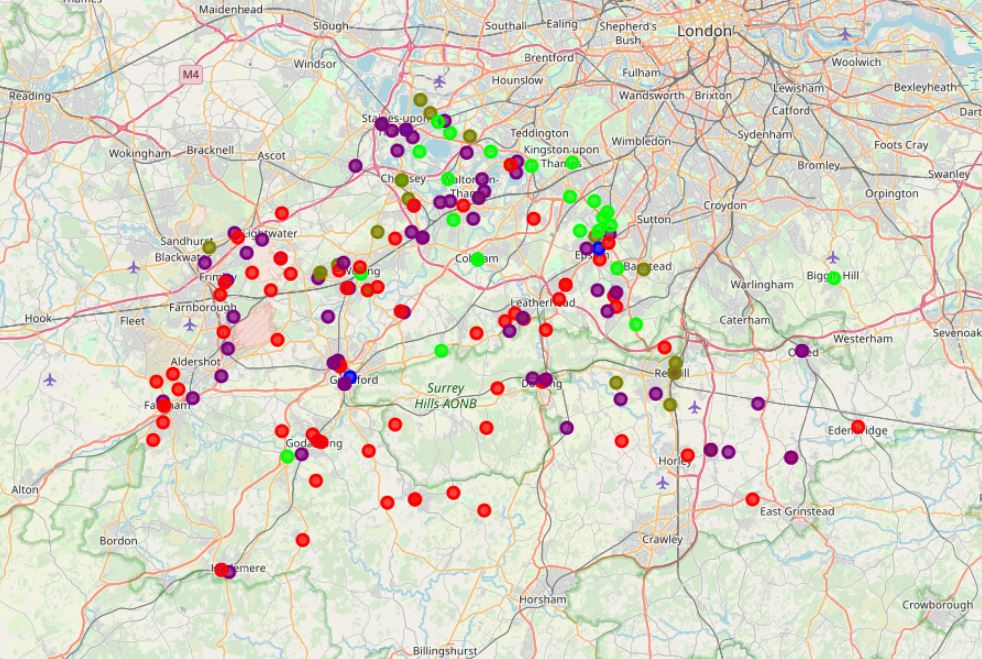
\includegraphics[width=\textwidth]
        {figures/ClustersOnMap.jpg}}
        \caption{\label{fig:map} visualisation of the clusters on the map}
      \end{figure}


Cluster 1, which includes wards in the centre of two big towns in Surrey area (i.e., Guildford and Epsom), shows that more venues can cause more risk in the area. As the Table below shows the number of crime committed in this cluster are significantly high. On the other hand, Cluster 3, is associated with wards that have a very low density of venues and a slight risk in terms of crime committed. However, Cluster 4, despite having a low density of the venues, it has high risk where make these wards undesirable since they are neither enough popular nor enough safe. These wards are mostly inside the M25 or near big town such as Woking or Redhill. Cluster 2 and 0 are slightly similar. They are wards with moderate density and relatively moderate risk. However, as presented in Fig. \ref{fig:map}, Cluster 0 includes wards where mostly are located inside the M25 band which make increases in specific categories of crime such as theft handling and vehicle interference in these areas. 
 \textit{In general, the model confirms we should expect crime rises in the more busy/popular areas. } 
 
 

 \begin{table}[ht]
\caption{Summary of Clusters' Data} % title of Table
\centering % used for centering table
\begin{tabular}{c c c c c } % centered columns (4 columns)
\hline\hline %inserts double horizontal lines
Cluster & \# of venues & Total Notifiable Offence &  Theft handling& vehicle interference  \\ [0.5ex] % inserts table
%heading
\hline % inserts single horizontal line
0 &  42  &  474 &  114& 13\\ % inserting body of the table
1 &78 & 1860 & 723&6\\
2 & 39  & 474 &  93&4\\
3 &  28 & 207 &35&3 \\
4 &  34 & 983 & 231&8\\ [1ex] % [1ex] adds vertical space
\hline %inserts single line
\end{tabular}
\label{tb:SummaryofClusters} % is used to refer this table in the text
\end{table}

\section{Conclusions}\label{conclusions}
 In this study, I investigated the relationship between the number/categories of venues and the number/categories of crime in different wards in Surrey county, UK. To precisely answer this question, I realised that I need more historical data related to the development of the venues and crime committed in this area. But utilising clustering technique, I was able to group different wards in unique clusters based on venues and crime features in those areas. This analysis helps us to have a better understanding of the different wards. 
\\\indent I built the \emph{k}-mean clustering model and examined different features in the model, such as the number of clusters as well as features in Foursquare such as limit and radios. I identified 5 clusters with unique features. These models can be instrumental in helping people to buy property in the Surrey county and are concern about the accessibility of the house to the restaurant club or night-life and safety of the area. For example, the result shows that areas in cluster 3 are very suitable for people who are looking for a quiet place with a high degree of safety. 



\end{document}

begin{itemize}
  
   \item  {\textbf{Cluster 0}: Low density \& Moderate risk}
   \item  {\textbf{Cluster 1}: Very high density \& Very high risk}
   \item {\textbf{Cluster 2}: Very low density \&  Very low risk }
  \item {\textbf{Cluster 3}: Moderate density\& high risk} 
  \item {\textbf{Cluster 4}: High density \& Moderate risk}
  
  
\end{itemize}